\section{Antenna Basics}
\subsection{High-Frequency Parameters}
\begin{itemize}
    \itemsep0pt
    \item Input reflection coefficient:\\
        \[r \text{ or } \Gamma = S_{11} = \dfrac{Z - Z_0}{Z + Z_0} = -\dfrac{Y - Y_0}{Y + Y_0}\]
    \item Current and Voltage stop being useful for high frequencies\\
        $\implies$ Power wave amplitudes $a$ and $b$:
    \begin{align*}
        &a = \dfrac{U_{in} + I_{in}Z_0}{2\sqrt{Z_0}} & U_{in} = \sqrt{Z_0} (a + b)\\
        &b = \dfrac{U_{in} - I_{in}Z_0}{2\sqrt{Z_0}} & I_{in} = \dfrac{a - b}{\sqrt{Z_0}}
    \end{align*}
    \item Much like Current and Voltage, Impedance Matrices also stop making sense at higher frequencies\\
    $\implies$ Scattering matrix $S$:
        \[\begin{bmatrix}b_1\\ b_2\end{bmatrix} =\
            \begin{bmatrix}S_{11} & S_{12}\\ S_{21} & S_{22}\end{bmatrix} \
            \begin{bmatrix}a_1\\ a_2\end{bmatrix}\]
    \item Characteristics of the far-field:
        \begin{itemize}
            \itemsep0pt
            \item spherical wave fronts
            \item work with locally plane waves
            \item no reactive fields (\(\mathrm{Im}\{\vec{S}\} = 0\))
            \item \(|\vec{k}| = \omega \sqrt{\epsilon\mu}\), TEM-propagation
        \end{itemize}

\end{itemize}

\subsection{Power in Antenna Systems}
There are several important definitions of power in antenna systems.
These include maximum generator power, accepted power, radiated power.
\todo{graphic for showing power flow}

\subsubsection{Maximum Generator Power}
Maximum generator power $P_{t0, \text{max}}$ is the total power provided by the generator (in a transmitter configuration).
This could e.g.\ be a transmitter generator for broadcast.

\subsubsection{Accepted Power}
Accepted power $P_{\text{t0}}$ that arrives at the antenna, after accounting for mismatch losses, i.e.\
\begin{equation*}
  P_{\text{t0}} = (1 - |\Gamma|^{2}) \, P_{\text{t0, max}}.
\end{equation*}

\subsubsection{Radiated Power}
Radiated power $P_{t}$ is the power that's emitted by the antenna as EM-waves:

\begin{equation*}
    P_t = \eta_a P_{t0} = \eta_{\text{tot}} \, P_{\text{t0, max}},
\end{equation*}

\begin{equation*}
  P_{t} = \oiint\limits_{\Omega} U \,\mathrm{d}\Omega = \iint\ \dfrac{{|E_{\text{max}}|}^{2}}{2 Z_{\text{F0}}} r^{2}\sin\vartheta \: \mathrm{d}\vartheta\mathrm{d}\varphi.
\end{equation*}


\subsection{Fundamental Antenna Parameters}
\subsubsection{Antenna Pattern (Characteristic)}
The characteristic $C(\vartheta, \varphi)$ is the angle-dependant antenna radiation under far-field conditions, normalized according to the maximum value.
    \begin{equation*}
        C(\vartheta, \varphi) = \dfrac{E(\vartheta, \varphi)}{E_{max}}, \quad
        |C(\vartheta, \varphi)| = \sqrt{\dfrac{S(\vartheta, \varphi)}{S_{max}}}
    \end{equation*}
\subsubsection{Beamwidth}
Beamwidth is beamwidth. Nuff' said.

\subsubsection{Radiation Power Density}
Describes the instantaneous power associated with an electromagnetic wave via the \textit{Poynting vector} $\vec{S}$.

\noindent In the far-field:
\begin{equation*}
    S(r) = \dfrac{|E(r)|^2}{2 Z_{F0}},\;\; Z_{F0} \approx \SI{377}{\Omega}
\end{equation*}
and for reciprocal antennas:
\begin{equation*}
    S(r) = \dfrac{P_{t0}G_t}{4\pi r^2} = \dfrac{P_{t0}\eta D_t}{4\pi r^2}.
\end{equation*}

\subsubsection{Radiation Intensity}
Radiation intensity in a given direction is the power radiated from an antenna per unit solid angle, i.e.\ it's a far-field value:
\begin{equation*}
  U(r) = r^{2}\,S(r) = r^{2} \dfrac{{|E(r)|}^{2}}{2 Z_{F0}}.
\end{equation*}

The total radiated power can be calculated from the radiation intensity as follows:
\begin{equation*}
  P_{t} = \oiint\limits_{\Omega} U \,\mathrm{d}\Omega = \int\limits_{\varphi=0}^{2\pi} \int\limits_{\vartheta=0}^{\pi} U \sin\vartheta \, \mathrm{d}\vartheta\mathrm{d}\varphi
\end{equation*}

\subsubsection{Directivity}
Directivity is the ratio of radiation in a specific direction compared to the (completely theoretical) isotropic radiator that radiates equally in all directions:

\begin{equation*}
 D = D(\vartheta, \varphi) = \dfrac{U(\vartheta, \varphi)}{U_{0}} = \dfrac{4\pi\,U(\vartheta, \varphi)}{P_{t}}.
\end{equation*}

If the direction isn't specified, then the direction of maximum radiation intensity is implied:
\begin{equation*}
D_{\mathrm{max}} = D_{0} = \dfrac{U}{U_{0}} = \dfrac{4\pi \, U_{\mathrm{max}}}{P_{t}}.
\end{equation*}

\subsubsection{Antenna Efficiency and Gain}
Total efficiency $\eta_{\mathrm{tot}}$ takes all losses from the generator to the emitted EM-waves into account
\begin{equation*}
  \eta_{{\mathrm{tot}}} = \underbrace{(1 - |\Gamma|^{2})}_{\text{mismatch loss}} \, \eta_{\mathrm{a}}, \quad \eta_{\mathrm{a}}:\text{antenna eff.}
\end{equation*}

As for the gain, there are two definitions: IEEE or absolute gain $G$ and realized gain $G_{\mathrm{realized}}$
\begin{align*}
  &G = \eta_{\mathrm{a}}D,\\
  &G_{\mathrm{realized}} = \eta_{\mathrm{tot}}D = (1 - |\Gamma|^{2})\,G.
\end{align*}

Notice that $G \geq G_{\mathrm{realized}}$.

    \begin{itemize}
    \item \textit{Effective area} $A_e$ and \textit{maximum effective area} (aperture) $A_0$ of reveiving antennas:\\
        \begin{align*}
            &A_e = \dfrac{P_{r,\mathrm{max}}}{S}\\
            &A_0 = \dfrac{P_{r0,\mathrm{max}}}{S}\\
            &P_{r0,\mathrm{max}}\text{: Maximum received power}
        \end{align*}
    \item For a \textit{reciprocal antenna} $\leftrightarrow$, the following holds:
        \begin{align*}
            A_0 &= \dfrac{\lambda_0^2}{4\pi} D &C_t(\vartheta, \varphi) = C_r(\vartheta, \varphi)\\
            A_e &= \dfrac{\lambda_0^2}{4\pi} G = \eta A_0&
        \end{align*}
    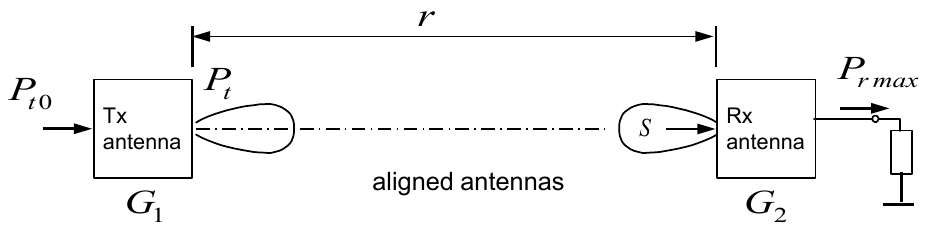
\includegraphics[width=.3\paperheight]{content/aawp/pictures/friis_transmission.png}
    \item \textbf{Friis Transmission Formula} for a radio link under far-field conditions:
        \begin{align}
            &\dfrac{P_{0,\text{RX}}}{P_{\text{A,TX}}} = G_{\text{TX}} G_{\text{RX}} \left(\dfrac{\lambda_0}{4\pi r} \right)^2,\label{eq:friis}\\
            &r: \text{distance between antennas},\nonumber\\
            &\lambda_0: \text{transmission wavelength},\nonumber\\
            &G_{\text{TX}}: \text{transmission antenna gain},\nonumber\\
            &G_{\text{RX}}: \text{receiving antenna gain}\nonumber
        \end{align}
    \item Radio Link Attenuation (\textit{Pathloss of free space}):\\
        \(\dfrac{a_0}{\si{dB}} = 10 \log_{10}^2\left(\dfrac{4 \pi r}{\lambda_0}\right) =\
        22 + 20 \log_{10}\left(\dfrac{r}{\lambda_0}\right)\)
\end{itemize}

\noindent\fbox{%
    \parbox{8cm}{%
        \textbf{How to Calculate Radiation Resistance} $R_r$:
        \begin{enumerate}
            \item Determine the antenna's current $I_a$ or its voltage $U_a$.
                \begin{equation*}
                    P_t = \dfrac{1}{2} |I_a|^2 R_r = \dfrac{1}{2} \dfrac{|U_a|^2}{R_r}
                \end{equation*}
            \item Equate the following with the above equation and solve for $R_r$:
                \begin{equation*}
                    P_t = \iint\limits_A \vec{S}(\vec{r}) \,\mathrm{d}\vec{A} = \iint\limits_A \dfrac{|E_{\mathrm{max}}|^2}{2 Z_F} |C(\vartheta,\varphi)|^2 \,\mathrm{d}\vec{A}
                \end{equation*}
        \end{enumerate}
    }}
